\subsection{Backend Aggregator}
\label{sec:backend-aggregator}
Once the data is published through HTTP POST, the back-end aggregator is then in charge of archiving such data and republishing to any connected browser for real time display. 

In order to seamless intergrate sMAP service, we choose to use JSON format with the following schema shown in the example. \texttt{DisplayName} is used to shown the name on web page, while \texttt{UniqueName} is used to maintain a hash table, mapping users to their physical location. \texttt{Readings} are the real data which contains both the UNIX timestamp and the room ID. Since sMAP is a general aggregator, \texttt{uuid} is used to select this stream of data.
\begin{lstlisting}
{
  "location" : {
    "DisplayName" : "Ben Zhang",
    "UniqueName" : "ee149.benzhang",
    "Readings" : [[1352756398000, 72]],
    "uuid" : "d8401a6e-2313-11e2-99e6-b8f6b119696f"
  }
}
\end{lstlisting}

As has shown in Sec.\,\ref{sec:system-architecture}, a middleware is necessary to interface with traditional browser. Previously we use {\em node.js} server for both static file hosting and real-time data pushing. But learning from most traditional approach that large static files (such as images and videos) are usually hosted on another domain/server to distribute the burden and improve reliability, we decided also to seperate these two tasks to provide higher reliability. All the html, css, js files and images are hosted using an Apache server, which is easy to config and set up. The node.js server starts by listening on any Socket.IO connection and once the connection is established, it registers itself as a subscriber of sMAP data stream. The real-time feed is then pushed back through Socket.io to the connected browser.

The front-end browser uses HTML5 Canvas element to draw the real-time location information. The major code which takes charge of such rendering is \texttt{parse.js} and \texttt{showMap.js}. \texttt{parse.js} maintains a list of mappings from room ID to the physical position (Point structure), and computes those locations whenever new data comes. \texttt{showMap.js} refreshes the entire drawing of the canvas when new data is coming using the mapped points. 

Other related information and links are also part of the web page, but such implementation was without too much technical challenges. One screenshot is provided in Fig.\,\ref{fig:webpage}.
\begin{figure}
  \centering
  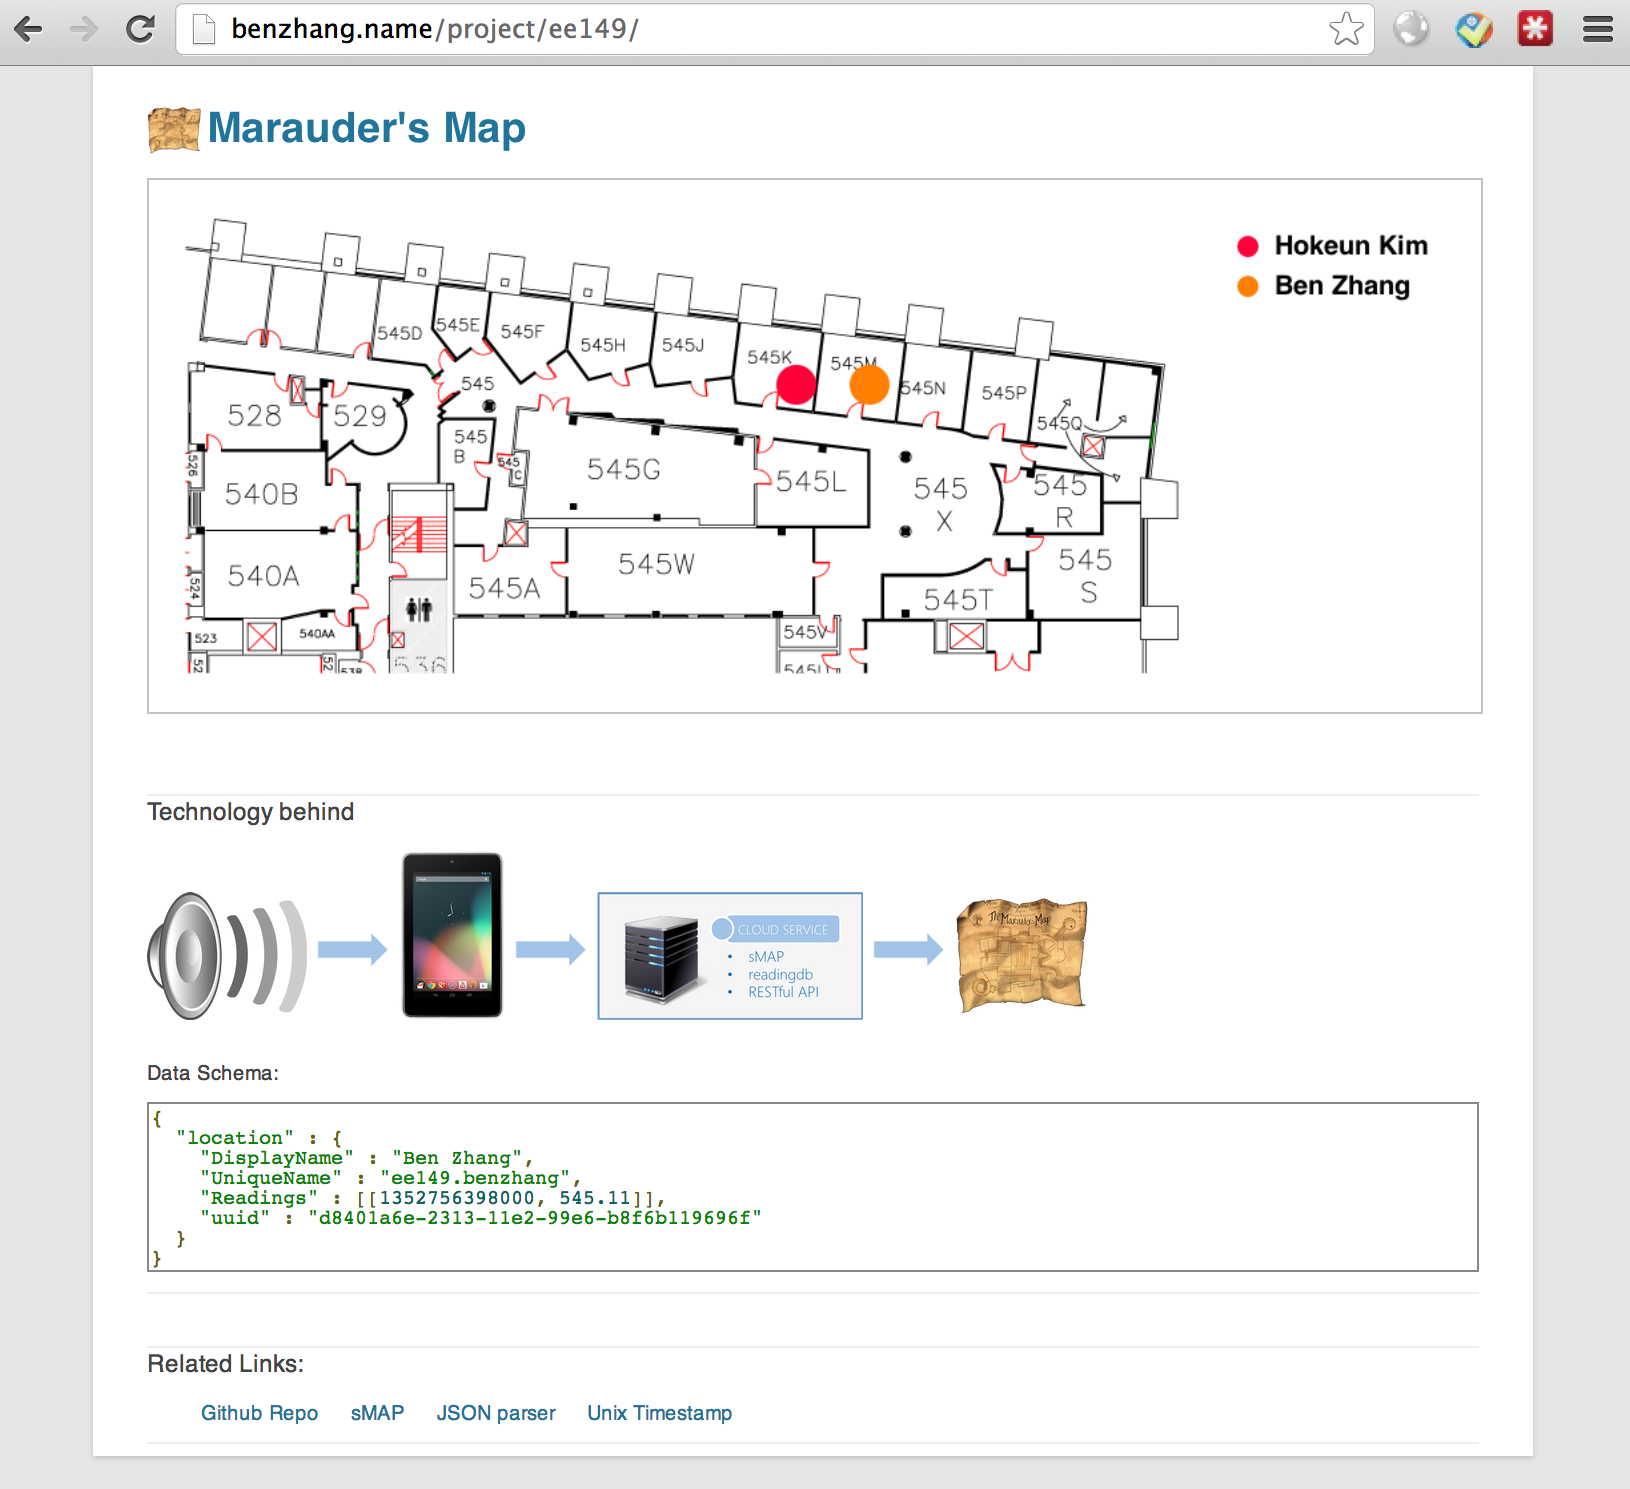
\includegraphics[width=0.8\columnwidth]{webpage}
  \caption{A screenshot of the webpage front-end}
  \label{fig:webpage}
\end{figure}


%% Master
%%% Local Variables: 
%%% mode: latex
%%% TeX-master: "ee149"
%%% End: 
